%%
%% Copyright 2022 OXFORD UNIVERSITY PRESS
%%
%% This file is part of the 'oup-authoring-template Bundle'.
%% ---------------------------------------------
%%
%% It may be distributed under the conditions of the LaTeX Project Public
%% License, either version 1.2 of this license or (at your option) any
%% later version.  The latest version of this license is in
%%    http://www.latex-project.org/lppl.txt
%% and version 1.2 or later is part of all distributions of LaTeX
%% version 1999/12/01 or later.
%%
%% The list of all files belonging to the 'oup-authoring-template Bundle' is
%% given in the file `manifest.txt'.
%%
%% Template article for OXFORD UNIVERSITY PRESS's document class `oup-authoring-template'
%% with bibliographic references
%%

%%%CONTEMPORARY%%%
\documentclass[unnumsec,webpdf,contemporary,large]{oup-authoring-template}%
%\documentclass[unnumsec,webpdf,contemporary,large,namedate]{oup-authoring-template}% uncomment this line for author year citations and comment the above
%\documentclass[unnumsec,webpdf,contemporary,medium]{oup-authoring-template}
%\documentclass[unnumsec,webpdf,contemporary,small]{oup-authoring-template}

%%%MODERN%%%
%\documentclass[unnumsec,webpdf,modern,large]{oup-authoring-template}
%\documentclass[unnumsec,webpdf,modern,large,namedate]{oup-authoring-template}% uncomment this line for author year citations and comment the above
%\documentclass[unnumsec,webpdf,modern,medium]{oup-authoring-template}
%\documentclass[unnumsec,webpdf,modern,small]{oup-authoring-template}

%%%TRADITIONAL%%%
%\documentclass[unnumsec,webpdf,traditional,large]{oup-authoring-template}
%\documentclass[unnumsec,webpdf,traditional,large,namedate]{oup-authoring-template}% uncomment this line for author year citations and comment the above
%\documentclass[unnumsec,namedate,webpdf,traditional,medium]{oup-authoring-template}
%\documentclass[namedate,webpdf,traditional,small]{oup-authoring-template}

%\onecolumn % for one column layouts

%\usepackage{showframe}

\graphicspath{{Fig/}}
\usepackage{eso-pic}
\usepackage{amsmath} 
\usepackage{graphicx}
\usepackage{color}
\usepackage{background}
\backgroundsetup{contents={}}
\usepackage{array}
\usepackage{booktabs}
\usepackage{tabularx}
\usepackage{longtable}
\usepackage{adjustbox}
\usepackage{ragged2e}
\newcolumntype{L}{>{\RaggedRight\arraybackslash}X}


% line numbers
%\usepackage[mathlines, switch]{lineno}
%\usepackage[right]{lineno}

\theoremstyle{thmstyleone}%
\newtheorem{theorem}{Theorem}%  meant for continuous numbers
%%\newtheorem{theorem}{Theorem}[section]% meant for sectionwise numbers
%% optional argument [theorem] produces theorem numbering sequence instead of independent numbers for Proposition
\newtheorem{proposition}[theorem]{Proposition}%
%%\newtheorem{proposition}{Proposition}% to get separate numbers for theorem and proposition etc.
\theoremstyle{thmstyletwo}%
\newtheorem{example}{Example}%
\newtheorem{remark}{Remark}%
\theoremstyle{thmstylethree}%
\newtheorem{definition}{Definition}

\begin{document}
\AddToShipoutPictureBG*{%
  \AtPageUpperLeft{%
    \put(10,-100){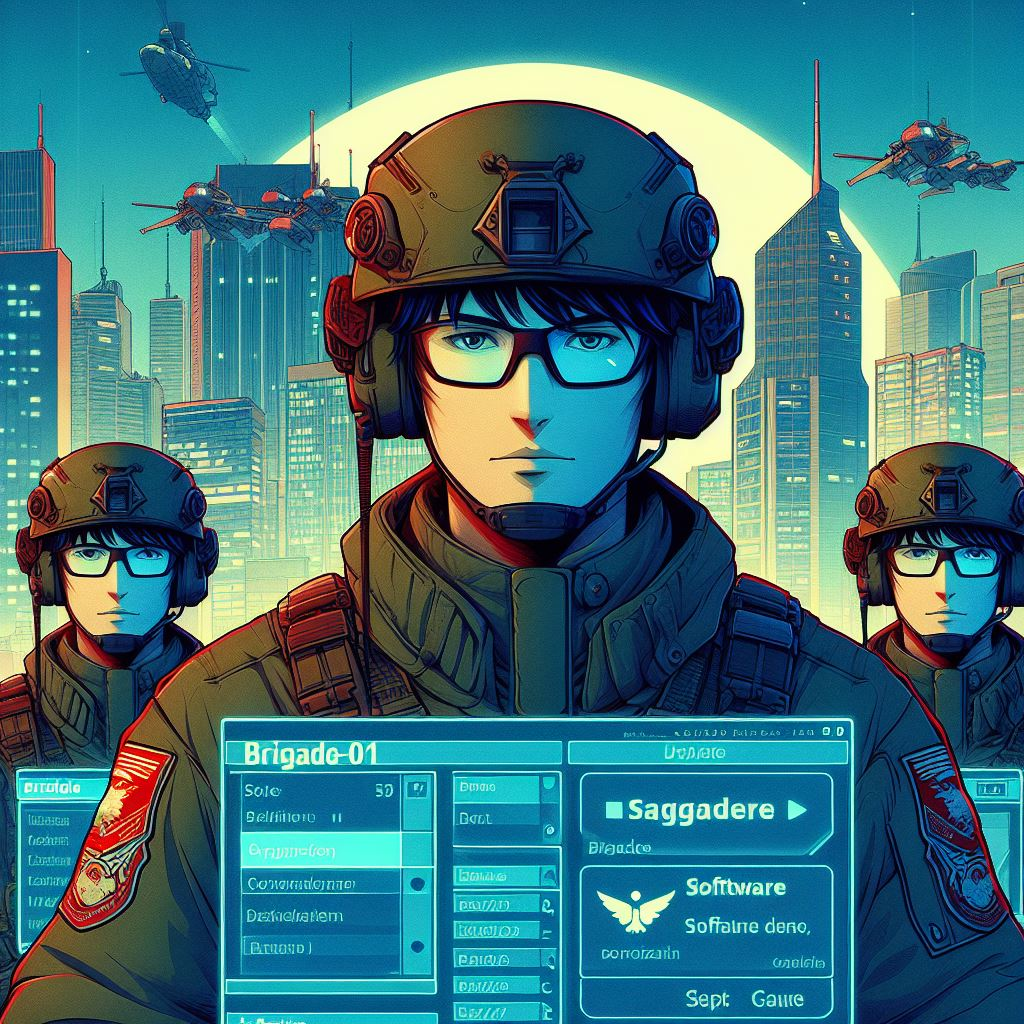
\includegraphics[width=1.93cm]{OIG3.jpg}}
  }%
}

\journaltitle{Brigade-01 | Big Data Management Technologies}
\copyrightyear{2024}
\pubyear{2024}
\access{\textbf{Github Repository: https://github.com/Brigade-01/Big-Data}}
\appnotes{Report}

\firstpage{1}

%\subtitle{Subject Section}

\title[Brigade-01]{Big Data Management Technologies}

\author[1$\ast$]{Spyridon Eftychios Kokotos}
\author[2$\ast$]{Florian Dima}
\author[3$\ast$]{Nikolaos Balatos}


\authormark{Spyridon Eftychios Kokotos et al.}

\address[1,2,3]{{\medium\orgdiv{Department of Informatics}}, {\medium\orgname{Ionian University}}, {\medium\orgaddress{\street{7, Tsirigoti Square}, \postcode{49100}, \state{Ionioi Nisoi}, \country{Greece}}}}

\corresp[$\ast$]{{\medium\textbraceleft skokotos - inf2021098, inf2021044, inf2021151\textbraceright}@ionio.gr}






\received{Date}{0}{Year}
\revised{Date}{0}{Year}
\accepted{Date}{0}{Year}


%\editor{Associate Editor: Name}

%\abstract{
%\textbf{Motivation:} .\\
%\textbf{Results:} .\\
%\textbf{Availability:} .\\
%\textbf{Contact:} \href{name@email.com}{name@email.com}\\
%\textbf{Supplementary information:} Supplementary data are available at \textit{Journal Name}
%online.}


\abstract{This project focuses on building a web-based application for data mining and analysis, leveraging either Streamlit or RShiny. Key features include tabular data loading, structured representation, 2D visualization, machine learning algorithm comparison, comprehensive result analysis, and project information. Also, this project aims to provide a user-friendly interface for in-depth data exploration and algorithm evaluation, catering to a wide audience.}
\keywords{Data Mining, Data Analysis, 2D Visualization, Machine Learning}

% \boxedtext{
% \begin{itemize}
% \item Key boxed text here.
% \item Key boxed text here.
% \item Key boxed text here.
% \end{itemize}}

\maketitle


\section{Introduction}
 As part of the \textbf{Big Data Management Technologies} course for the academic year 2023-2024, this project involves the development of a sophisticated web-based data analysis application utilizing machine learning (ML) algorithms. The primary aim is to create a comprehensive platform capable of processing tabular data, applying various ML algorithms, and providing detailed comparative analysis of their accuracy and performance. 
\vspace{0.3cm}

The primary objective of this project is for students to leverage existing online code resources to develop a sophisticated, user-centric application. This application will be designed to accept tabular data, process it through multiple machine learning algorithms, and output the corresponding results. Additionally, the application will compare the accuracy levels of each algorithm, providing a comprehensive analysis of their performance.


\section{Design of the Application}\label{sec2}

The implemented application encompasses a range of sophisticated features tailored for comprehensive data analysis and visualization. It offers a user-friendly interface facilitating seamless exploration of datasets. Within its framework, users can access a dedicated 2D Visualization Tab, enabling data visualization through advanced algorithms such as PCA and t-SNE, alongside the presentation of Exploratory Data Analysis (EDA) plots. 
\vspace{0.3cm}

Furthermore, the Classification Tab empowers users to execute data classification tasks utilizing robust algorithms like Random Forest and SVC (Support Vector Classifier), while the Clustering Tab facilitates data grouping through the application of K-Means and Agglomerative Clustering algorithms, thus enhancing the depth and efficiency of data processing and interpretation.

\section{Information about the Tabs}\label{subsec1}
\vspace{0.3cm}

\subsection{\textbf{2D Visualization Tab}}
\vspace{0.2cm}

Exploratory Data Analysis (EDA) diagrams are visual tools used to summarize the main characteristics of a dataset, often with visual methods. These diagrams play a critical role in data analysis by helping to uncover underlying patterns, detect anomalies, test hypotheses, and check assumptions through a graphical representation. Common types of EDA diagrams include histograms, box plots, scatter plots, and bar charts, each serving different purposes such as displaying distribution, variability, relationships, and categorical data insights. 
\vspace{0.2cm}

By transforming raw data into visual formats, EDA diagrams facilitate a better understanding of the data's structure and guide subsequent analytical or modeling steps, ensuring a robust and informed approach to data science and statistical analysis.
\vspace{0.2cm}

A Box Plot, or whisker plot, displays data distribution based on a five-number summary: minimum, first quartile (Q1), median, third quartile (Q3), and maximum. It highlights central tendency, spread, and skewness, and identifies outliers, making it easy to compare distributions across different datasets.
\vspace{0.2cm}

A Density Diagram, or density plot, provides a smoothed curve that represents the probability distribution of a continuous variable. It offers a clear view of the data’s shape, central tendency, and variability without the noise of histogram bins.
\vspace{0.1cm}

Right above, you can find one of the many figures (that will be included in the report in a specific section at the end) related to the PCA algorithm.
\vspace{0.2cm}

A Heatmap uses color to represent the values of a matrix, allowing for a quick visual summary of data. It is useful for displaying correlations, identifying patterns, and highlighting areas of high or low intensity, simplifying complex data for easier interpretation.
\vspace{0.2cm}

\begin{figure}
    \centering
    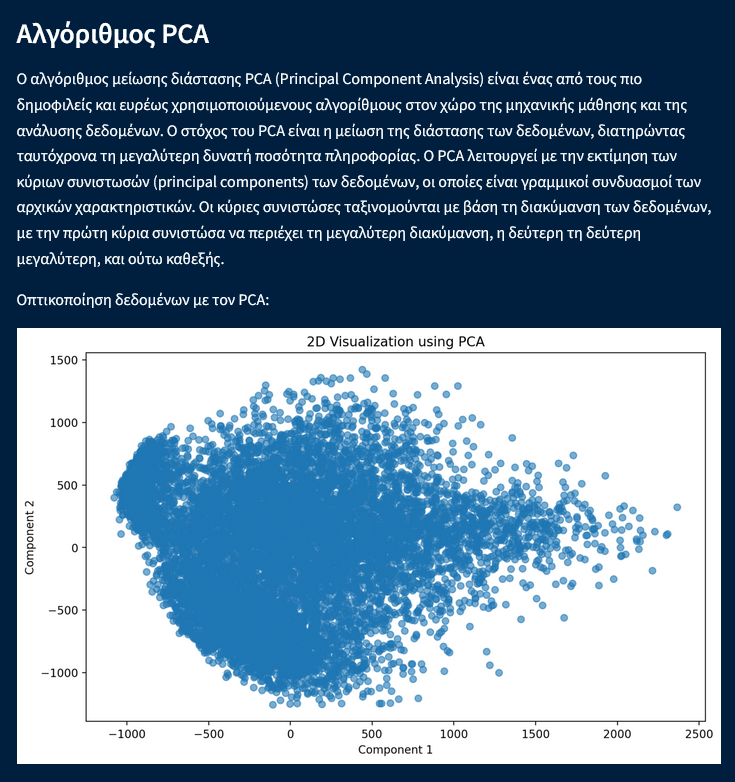
\includegraphics[width=0.4\linewidth]{pca.png}
    \caption{The results of visualization after processing them through the PCA algorithm.}
    \label{fig:pca}
\end{figure}

\subsection{\textbf{Classification Tab}}
\vspace{0.2cm}


The Classification Tab of the application showcases two powerful machine learning algorithms: Random Forest and Support Vector Classifier (SVC). Random Forest, a robust ensemble learning technique, is adept at making predictions and classifications by aggregating the outputs of multiple decision trees. Its strength lies in the diversity of these trees, which operate independently and combine their predictions to yield more accurate results. 
\vspace{0.2cm}

By mitigating overfitting and enhancing prediction accuracy, Random Forest effectively addresses various classification challenges. On the other hand, Support Vector Classifier (SVC) is a formidable algorithm for binary classification tasks. It endeavors to delineate data points in feature space using an optimal hyperplane, thereby creating a clear demarcation between classes. SVC's flexibility and efficacy in diverse classification scenarios, coupled with its resilience to high-dimensional data, render it a versatile tool for classification tasks. 
\vspace{0.2cm}

Through interactive interfaces, users can explore the intricacies of these algorithms, analyze their predictive performance, and gain valuable insights for decision-making and problem-solving.
\vspace{0.2cm}

It's imperative to note that in the categorization tab, the .csv file must incorporate the respective label for the process to advance, as it's deemed indispensable in machine learning. Consequently, if file upload is sanctioned without the inclusion of the label, the following error will manifest on the specific tab:

KeyError: 'label'

\begin{figure}
    \centering
    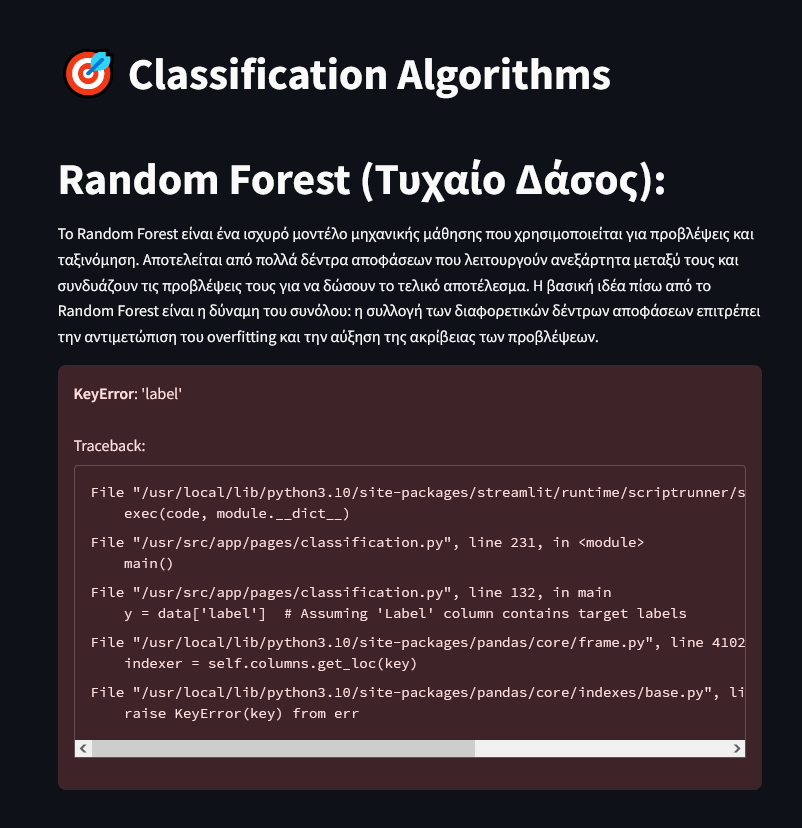
\includegraphics[width=0.4\linewidth]{error-classification.png}
    \caption{The \textbf{KeyError: 'label"} error that show no label was found in the .csv file}
    \label{fig:error-classification}
\end{figure}

\subsection{\textbf{Clustering Tab}}
\vspace{0.2cm}

The Clustering Tab of the application presents two clustering algorithms: K-Means and Hierarchical Clustering (Agglomerative Clustering). K-Means is a widely used unsupervised learning algorithm for partitioning data into a predetermined number of clusters. It iteratively assigns each data point to the nearest centroid, optimizing the centroid positions until convergence. K-Means finds applications in pattern recognition, group analysis, and as a preprocessing step for other algorithmic applications. 
\vspace{0.2cm}

On the other hand, Hierarchical Clustering constructs hierarchical groupings of data points. It starts by considering each data point as a separate cluster and then iteratively merges the closest clusters until a single cluster or the desired number of clusters is achieved. Hierarchical Clustering comes in two main types: Agglomerative, which starts with small clusters and merges them, and Divisive, which starts with one large cluster and divides it. 
\vspace{0.2cm}

Through interactive interfaces, users can explore these clustering algorithms, analyze their clustering results, and compare their performance using evaluation metrics such as Silhouette Score, Calinski-Harabasz Index, Davies-Bouldin Index, Dunn Index, and Between-Cluster Sum of Squares (BSS).


\section{Team Contributions \& Information Tab}\label{sec3}
\vspace{0.2cm}

In the Information tab, detailed insights regarding the developmental endeavors of the scientific mode are delineated. The team, spearheaded by \textbf{\textit{Florian Dima}}, encompasses pivotal tasks including the conceptualization of the \textbf{Clustering Tab}, crafting \textbf{UML Diagrams}, orchestrating the \textbf{Software Development Life Cycle}, and the formulation of \textbf{Dockerfile}. 
\vspace{0.1cm}

\textbf{\textit{Spyridon Eftychios Kokotos}} assumes a multifaceted role, spearheading the establishment of the \textbf{Brigade-01 Organization} and the \textbf{Big-Data repository} on \textbf{GitHub}, orchestrating the \textbf{Implementation of the Classification Tab}, and \textbf{facilitating seamless data integration from CSV to pertinent tabs}. Additionally, \textbf{\textit{Kokotos}} undertakes the onus of drafting \textbf{User Guidelines} and the \textbf{Final Report}. 
\vspace{0.2cm}

\textbf{\textit{Nikolaos Balatos}}, on the other hand, undertakes the technical implementations of the \textbf{2D Visualization} and \textbf{Home Tabs}, alongside infusing the \textbf{Info Tab} with requisite functionalities. Furthermore, \textbf{\textit{Balatos}} orchestrates the seamless \textbf{linkage of data from CSV to the Home and 2D Visualization Tabs}, complementing the efforts with \textbf{UML Diagrams} and the \textbf{Software Development Life Cycle} adherence.
\vspace{0.2cm}

\section{Agile Model for the Software Version Lifecycle of the Web-Based Data Mining and Analysis Application}
\vspace{0.2cm}

For the development of the web-based data mining and analysis application using Streamlit, we propose the utilization of the Agile model. The Agile model is characterized by its flexibility, enabling continuous improvement and adaptation through iterative development cycles (sprints) and continuous feedback loops. Below, we outline the key stages of the software version lifecycle based on Agile:
\vspace{0.2cm}

\paragraph{1. Initial Planning:}
\vspace{0.2cm}

\begin{itemize}
    \item \textbf{Requirement Gathering}: Collection of functional and non-functional requirements from stakeholders.
    \vspace{0.1cm}
    \item \textbf{Purpose and Goals Definition}: Determination of the application's overall purpose and the core goals to be achieved.
    \vspace{0.1cm}
    \item \textbf{Architectural Design:} Development of the application's architectural design, including UML diagrams.
\end{itemize}
\vspace{0.1cm}

\paragraph{2. Backlog Creation:}
\vspace{0.2cm}

\begin{itemize}
    \item \textbf{Product Backlog:} Recording of all requirements and features in the form of user stories in the product backlog.
    \vspace{0.1cm}
    \item \textbf{Sprint Backlog:} Selection of user stories to be completed in each sprint from the product backlog.
\end{itemize}
\vspace{0.1cm}

\paragraph{3. Sprint Planning:}
\vspace{0.2cm}

\begin{itemize}
    \item \textbf{Sprint Duration Definition:} Setting the duration of each sprint (typically 1-2 weeks).
    \vspace{0.1cm}
    \item \textbf{Sprint Goals:} Defining the sprint goals and the user stories to be completed.
\end{itemize}
\vspace{0.1cm}

\paragraph{4. Sprint Execution:}
\vspace{0.2cm}

\begin{itemize}
    \item \textbf{Development:} Implementation of the application's features and functionalities according to the user stories.
    \vspace{0.1cm}
    \item \textbf{Daily Stand-ups:} Daily team meetings to review progress and address any impediments.
\end{itemize}
\vspace{0.1cm}

\paragraph{5. Review and Feedback:}
\vspace{0.2cm}

\begin{itemize}
    \item \textbf{Sprint Review:} Presentation of sprint results to stakeholders and collection of feedback.
    \vspace{0.1cm}
    \item \textbf{Sprint Retrospective:} Review of the sprint process by the development team and identification of areas for improvement.
\end{itemize}
\vspace{0.1cm}

\paragraph{6. Continuous Integration and Delivery:}
\vspace{0.2cm}

\begin{itemize}
    \item \textbf{Code Integration:} Continuous integration of new code into the central repository and execution of automated tests.
    \item \textbf{Delivery:} Delivery of the completed functionality at the end of each sprint.
\end{itemize}
\vspace{0.1cm}

\paragraph{7. Evaluation and Improvement:}
\vspace{0.2cm}

\begin{itemize}
    \item \textbf{Metrics Analysis:} Evaluation of algorithm and application performance based on performance metrics.
    \item \textbf{Continuous Improvement:} Implementation of enhancements based on feedback and analysis results.
\end{itemize}
\vspace{0.1cm}

\paragraph{8. Final Release and Support}
\vspace{0.2cm}

\begin{itemize}
    \item \textbf{Release:} Creation of the final release of the application and delivery to end users.
    \item \textbf{Support:} Provision of support and maintenance for bug fixes and addition of new features.
\end{itemize}
\vspace{0.1cm}

Adaptation to Team Collaboration:

\begin{itemize}
    \item \textbf{GitHub Usage:} Code management and team collaboration through GitHub, utilizing pull requests and code reviews.
   \item \textbf{Docker:} Use of Docker for application development and deployment, ensuring consistency in development and production environments.
\end{itemize}

Final Conclusion:
\vspace{0.2cm}

The use of the Agile model enables the team to remain flexible and respond quickly to changes in requirements and user feedback. Through continuous feedback and iterative development cycles, it ensures that the final product fully meets user needs and is of high quality.

\section{Installation Instructions}
\vspace{0.2cm}

\paragraph{\textbf{Option 1}: Docker Image Pull:}
\vspace{0.2cm}

\textbf{1. Pull the Docker Image}
\vspace{0.2cm}

\begin{itemize}
    \item Retrieve the Docker image from Docker Hub by executing the following command in your terminal: `\textit{docker pull spyridonkokotos/big-data:latest}`
\end{itemize}
\vspace{0.2cm}

\textbf{2. Run the Docker Container}
\vspace{0.2cm}

\begin{itemize}
    \item Deploy the Docker container using the following command: `\textit{docker run -d --name big-data -p 8501:8501 spyridonkokotos/big-data:latest}
\end{itemize}
\vspace{0.2cm}

\textbf{3. Access the Application}
\vspace{0.2cm}

\begin{itemize}
    \item Open your preferred web browser and navigate to \textit{http://localhost:8501} to interact with the application.
\end{itemize}
\vspace{0.2cm}

\paragraph{\textbf{Option 2}: Build the local Dockerfile:}
\vspace{0.2cm}

\textbf{1. Clone the Repository}
\vspace{0.2cm}

\begin{itemize}
    \item Clone the repository from GitHub to your local machine using the following command: `\textit{git clone https://github.com/Brigade-01/Big-Data.git}`
\end{itemize}
\vspace{0.2cm}

\textbf{2. Navigate to the Project Directory:}
\vspace{0.2cm}

\begin{itemize}
    \item Change to the project directory where the source files are located: `\textit{cd Big-Data/src/}`
\end{itemize}
\vspace{0.2cm}

\textbf{3. Build the Docker Image:}
\vspace{0.2cm}

\begin{itemize}
    \item Construct the Docker image locally by executing: `\textit{docker build -t big-data:latest .}`
\end{itemize}
\vspace{0.2cm}

\textbf{4. Run the Docker Container:}
\vspace{0.2cm}

\begin{itemize}
    \item Deploy the Docker container with the following command: `\textit{docker run -d --name big-data -p 8501:8501 spyridonkokotos/big-data:latest}`
\end{itemize}
\vspace{0.2cm}

\textbf{5. Access the Application:}
\vspace{0.2cm}

\begin{itemize}
    \item Open your preferred web browser and navigate to http://localhost:8501 to interact with the application.
\end{itemize}
\vspace{0.2cm}

\section{Basic Usage:}\label{sec3}
\vspace{0.2cm}

To efficiently utilize the application for data analysis and algorithm comparison, begin by uploading your desired file. Select either a .csv or .xls file by clicking the "Browse Files" button. Await a confirmation message indicating the successful upload of your file. Upon successful upload and validation of the file's content, you may proceed to explore the application's features.
\vspace{0.2cm}

Navigate through the various tabs using the menu on the left side of the interface. This allows you to access different functionalities and apply included algorithms to test their performance on your dataset. This structured approach ensures a seamless and effective user experience within the application.


\section{Classification Results:}\label{sec3}
\vspace{0.2cm}

SVC performed better since the accuracy was slightly higher than for the random forest
\vspace{0.2cm}

\section{UML Diagrams:}\label{sec3}
\vspace{0.2cm}

\paragraph{Use Case Diagram:}
\vspace{0.2cm}

The Use Case Diagram presents a high-level view of the user's interaction with the web application, delineating the primary functionalities:
\vspace{0.2cm}

\begin{itemize}
    \item File Upload: The user initiates interaction by uploading a file, which is central to subsequent processes.
    \vspace{0.2cm}
    \item 2D Visualization: Once a file is uploaded, the user can generate 2D visualizations. This includes the generation of diagrams using dimensionality reduction algorithms and Exploratory Data Analysis (EDA).
    \vspace{0.2cm}
    \item Dimensionality Reduction Algorithms Diagrams: These diagrams simplify data for visualization purposes.
    \vspace{0.2cm}
    \item EDA Diagrams: These diagrams assist in initial data analysis by summarizing the main characteristics.
    \vspace{0.2cm}
    \item Machine Learning Implementation: The user can implement machine learning algorithms, which include:
\end{itemize}

\begin{enumerate}
    \item
    Clustering Algorithm Implementation: Algorithms such as hierarchical clustering and K-nearest neighbors (KNN) are utilized to group data points.
    \vspace{0.2cm}
    \item Classification Algorithm Implementation: Algorithms like Random Forest and Support Vector Classification (SVC) are used to classify data points
    \vspace{0.2cm}.
    \item Results \& Comparison Printing: The results from clustering and classification implementations are compared and printed for analysis.
\end{enumerate}

\paragraph{Class Diagram:}
\vspace{0.2cm}

The Class Diagram provides a detailed structural view of the application by defining its classes, attributes, and relationships:
\vspace{0.2cm}

\begin{itemize}
    \item FILE Class:
    Attributes:
        file size (up to 200MB)
        file type (supports .csv and .xlsx formats)
    This class is pivotal as it interfaces with other classes to provide the data required for processing.
    \vspace{0.2cm}
    \item 2D Visualization Class:
    Methods:
        TSNE(file): Applies t-Distributed Stochastic Neighbor Embedding for visualization.
        PCA(file): Applies Principal Component Analysis for dimensionality reduction.
        EDAdiagrams(file): Generates EDA diagrams to summarize data characteristics.
    \vspace{0.2cm}
    \item ML ALGORITHMS Class:
    Method:
        CompareResults(): Compares the results of different machine learning algorithms.
    This class acts as a parent class for clustering and classification algorithms.
    \item Clustering Algorithms Class (inherits from ML ALGORITHMS):
    Methods:
        HIER-CLUSTERING(file): Implements hierarchical clustering.
        KNN(file): Implements the K-nearest neighbors algorithm.
        CompareResults(results): Specific implementation of the result comparison.
    \vspace{0.2cm}
    \item Classification Algorithms Class (inherits from ML ALGORITHMS):
    Methods:
        RND-FOREST(file): Implements the Random Forest algorithm.
        SVC-CLASS(file): Implements the Support Vector Classification algorithm.
        CompareResults(results): Specific implementation of the result comparison.
\end{itemize}
\vspace{0.2cm}

These diagrams collectively elucidate the application's functionality and structure, illustrating the user interactions and the modular design of classes facilitating various data analysis and machine learning tasks. This detailed representation ensures clarity in understanding the workflow and integration of different analytical methods within the application.

\section{Reporting Bugs:}\label{sec3}
\vspace{0.2cm}

To report a discovered bug, it is imperative to open an issue on GitHub, as previously outlined. Accurate bug reporting is crucial for effective resolution and system improvement. When documenting a bug, please provide a detailed description, including steps to reproduce the issue, observed behavior, and expected behavior. 
\vspace{0.2cm}

Additionally, including relevant system information and any error messages encountered will facilitate a more efficient troubleshooting process. This systematic approach ensures that developers can quickly identify and address the problem, thereby enhancing the overall functionality and reliability of the software.


\section{License}
MIT License

\vspace{0,5em}

Copyright (c) 2024 Brigade-01
\vspace{0,5em}

Permission is hereby granted, free of charge, to any person obtaining a copy
of this software and associated documentation files (the "Software"), to deal
in the Software without restriction, including without limitation the rights
to use, copy, modify, merge, publish, distribute, sublicense, and/or sell
copies of the Software, and to permit persons to whom the Software is
furnished to do so, subject to the following conditions:

\vspace{0,5em}

The above copyright notice and this permission notice shall be included in all
copies or substantial portions of the Software.

\vspace{0,5em}

THE SOFTWARE IS PROVIDED "AS IS", WITHOUT WARRANTY OF ANY KIND, EXPRESS OR
IMPLIED, INCLUDING BUT NOT LIMITED TO THE WARRANTIES OF MERCHANTABILITY,
FITNESS FOR A PARTICULAR PURPOSE AND NONINFRINGEMENT. IN NO EVENT SHALL THE
AUTHORS OR COPYRIGHT HOLDERS BE LIABLE FOR ANY CLAIM, DAMAGES OR OTHER
LIABILITY, WHETHER IN AN ACTION OF CONTRACT, TORT OR OTHERWISE, ARISING FROM,
OUT OF OR IN CONNECTION WITH THE SOFTWARE OR THE USE OR OTHER DEALINGS IN THE
SOFTWARE.

\section{Authors contributions statement}
The above program is a creation of:

\vspace{0,5em} \textit{Florian Dima}, \textit{Nikolaos Balatos} \& \textit{Spyridon Eftychios Kokotos} 

and you can use it for your personal projects or further develop it as long as you always give credit to the creators.

\begin{table}[h]
\begin{tabularx}{\linewidth}{|L|L|L|L|L|} % Χρησιμοποιούμε το περιβάλλον tabularx και τον νέο τύπο στήλης L
\hline
\textbf{First Name} & \textbf{Last Name} & \textbf{Registry Number} & \textbf{Semester} & \textbf{Academic Email} \\
\hline
Florian & Dima & inf2021044 & 6th & inf2021044@ionio.gr \\
\hline
Nikolaos & Balatos & inf2021151 & 6th & inf2021151@ionio.gr \\
\hline
Spyridon - Eftychios & Kokotos & inf2021098 & 6th & \begin{tabular}[t]{@{}L@{}}inf2021098@ionio.gr \\ skokotos@ionio.gr\end{tabular} \\
\hline
\end{tabularx}
\caption{Contact Details of Students}
\label{tab:contact-details}
\end{table}

\section{Figures}

\begin{figure}
    \centering
    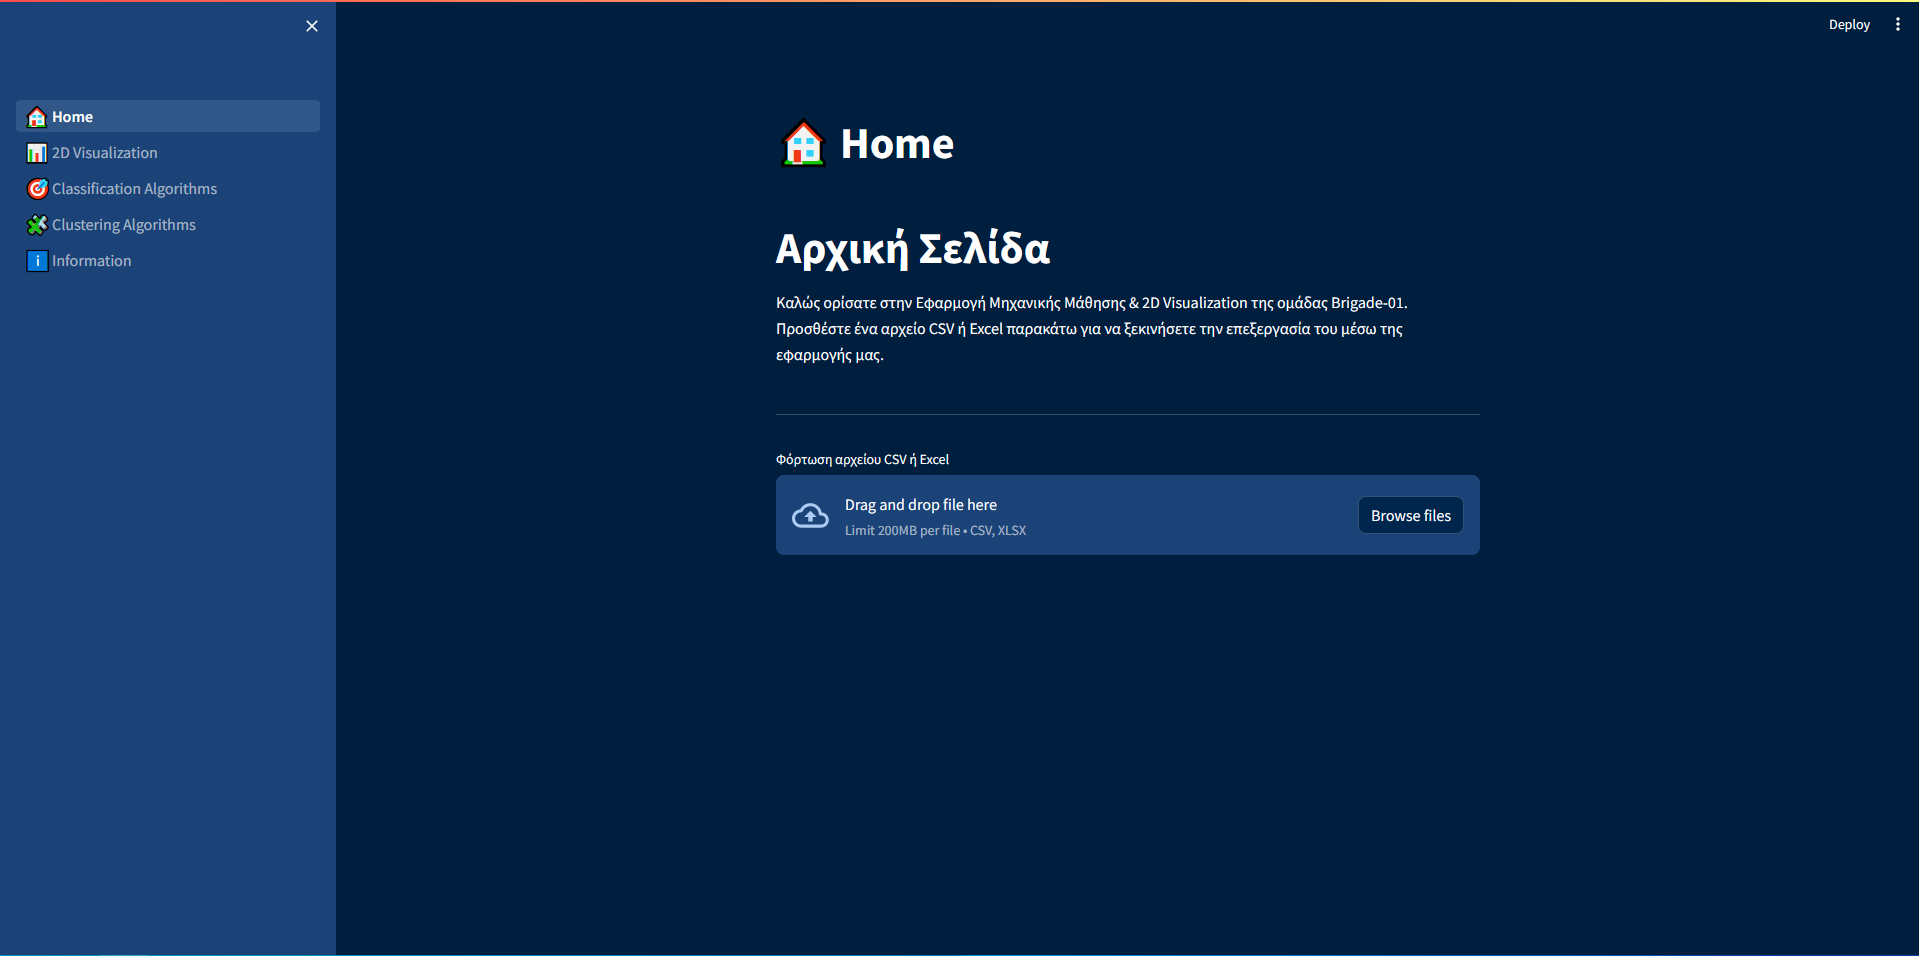
\includegraphics[width=1\linewidth]{welcoming-screen.png}
    \caption{Welcome Screen of the Application}
    \label{fig:welcome-screen}
\end{figure}

\begin{figure}
    \centering
    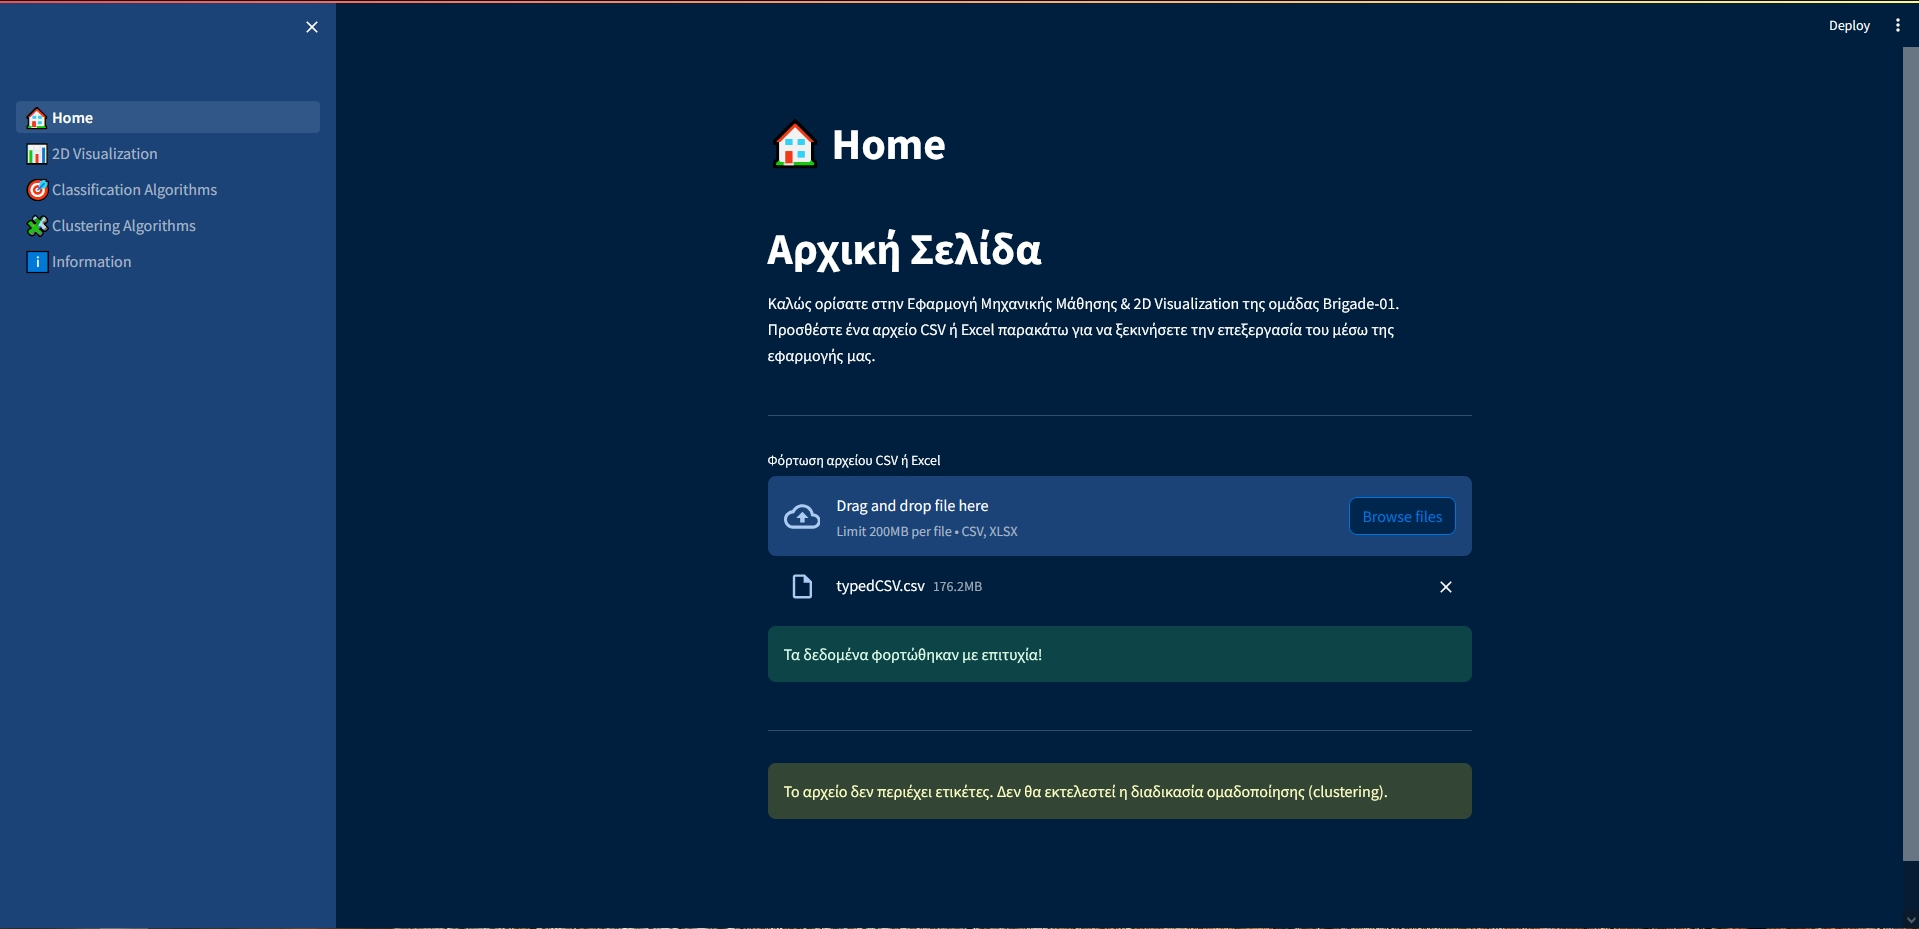
\includegraphics[width=1\linewidth]{csv-loaded.jpg}
    \caption{The Successful loading of the .csv dataset}
    \label{fig:csv-loaded}
\end{figure}

\begin{figure}
    \centering
    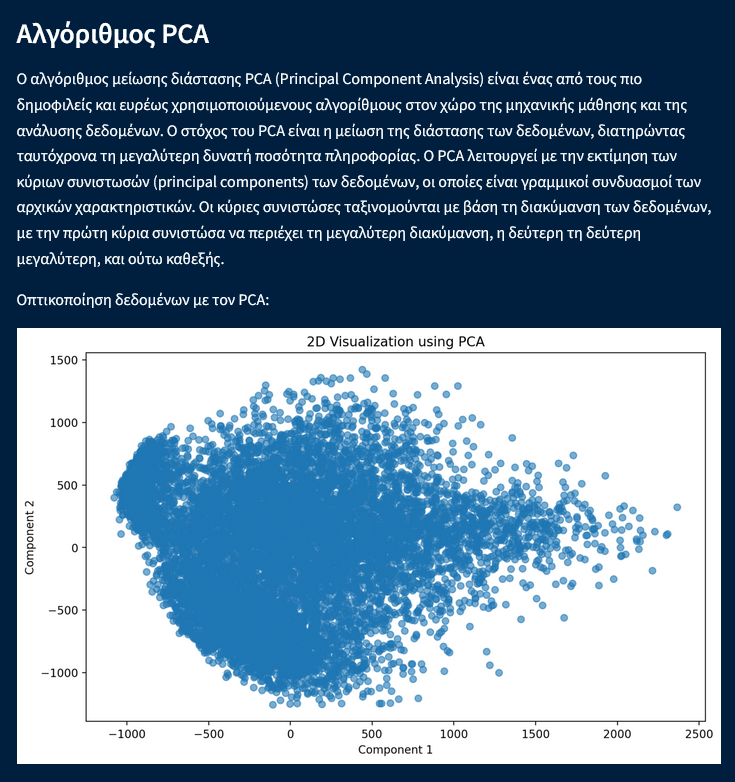
\includegraphics[width=0.9\linewidth]{pca.png}
    \caption{The results of visualization after processing them through the PCA algorithm}
    \label{fig:pca}
\end{figure}

\begin{figure}
    \centering
    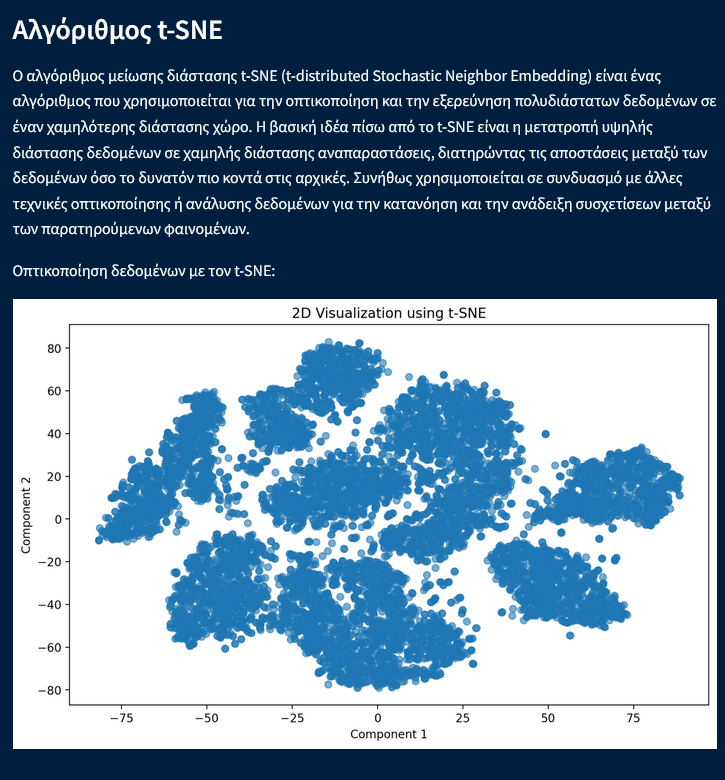
\includegraphics[width=1\linewidth]{t-sne.png}
    \caption{The results of visualization after processing them through the t-SNE algorithm}
    \label{fig:t-sne}
\end{figure}

\begin{figure}
    \centering
    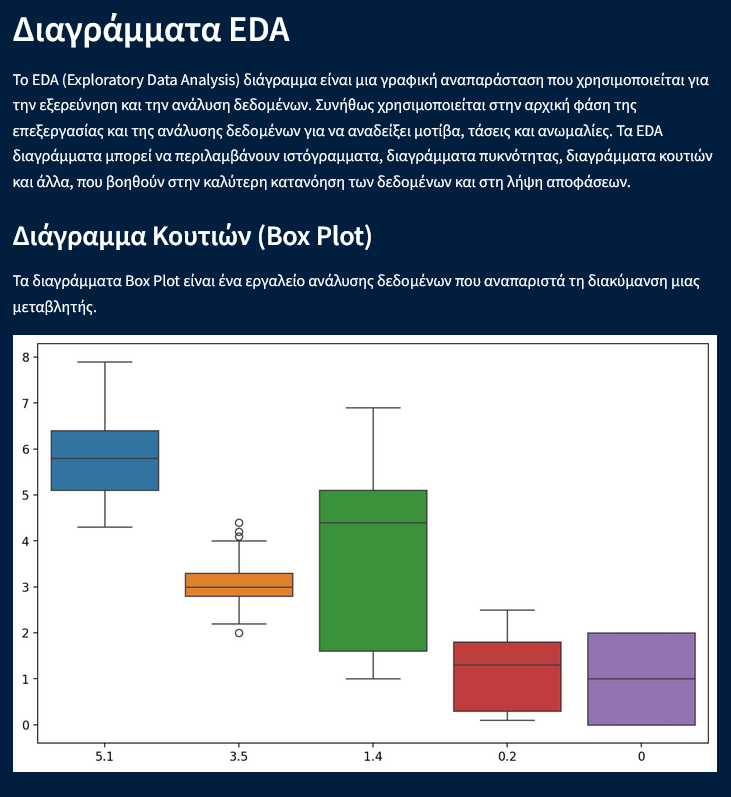
\includegraphics[width=1\linewidth]{eda-boxplot.png}
    \caption{EDA-Boxplot Diagram}
    \label{fig:eda-boxplot}
\end{figure}

\begin{figure}
    \centering
    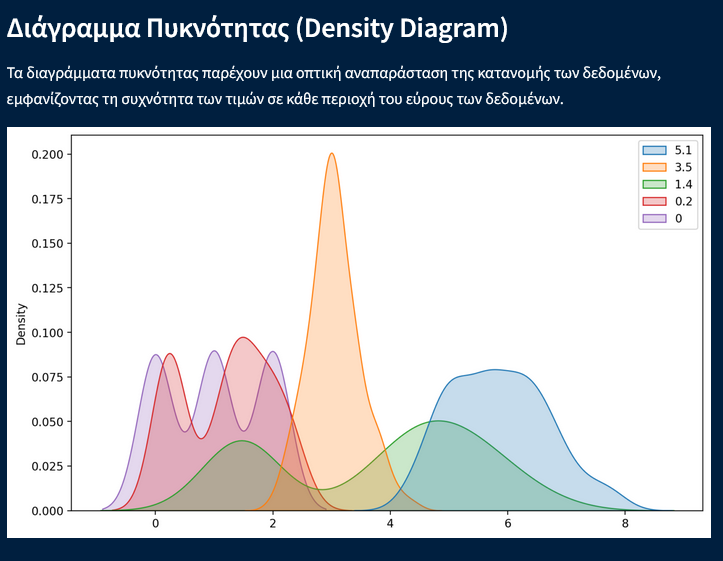
\includegraphics[width=1\linewidth]{density.png}
    \caption{Density Diagram}
    \label{fig:density}
\end{figure}

\begin{figure}
    \centering
    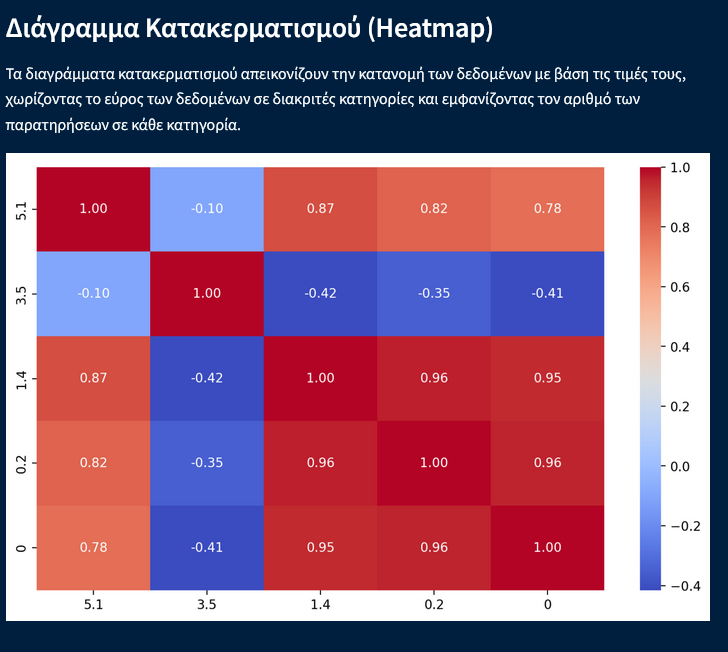
\includegraphics[width=1\linewidth]{heatmap.png}
    \caption{Heatmap Diagram}
    \label{fig:heatmap}
\end{figure}

\begin{figure}
    \centering
    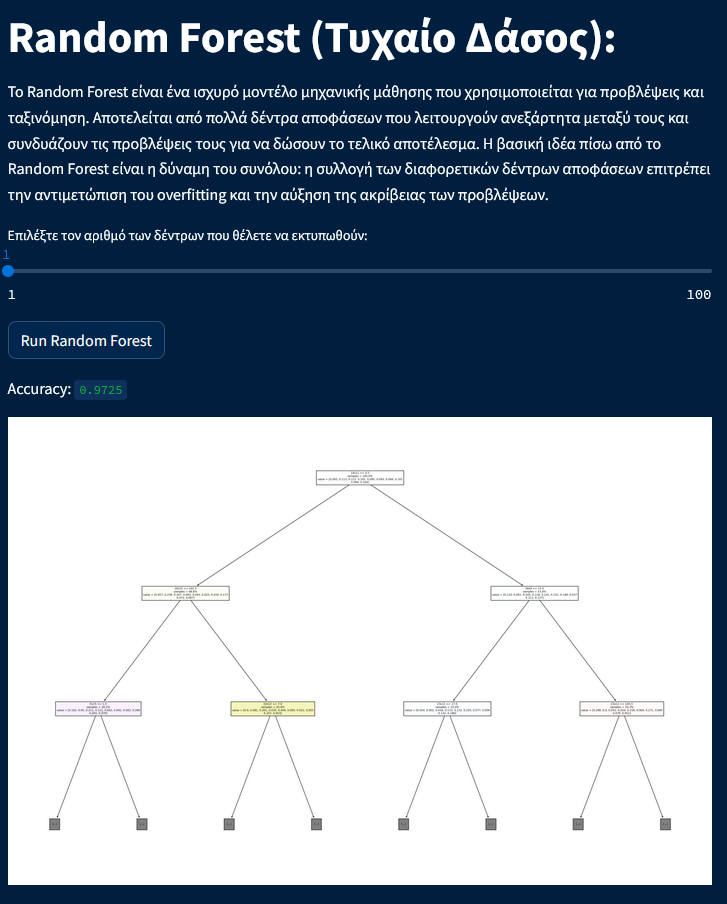
\includegraphics[width=1\linewidth]{random-forest.png}
    \caption{Random Forest Diagram}
    \label{fig:random-forest}
\end{figure}

\begin{figure}
    \centering
    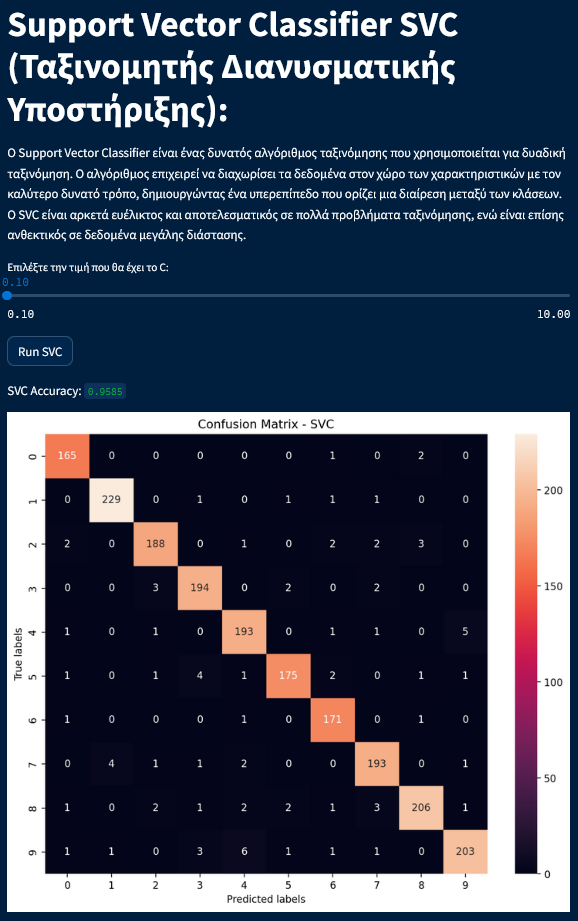
\includegraphics[width=1\linewidth]{svc.png}
    \caption{SVC Diagram}
    \label{fig:svc}
\end{figure}

\begin{figure}
    \centering
    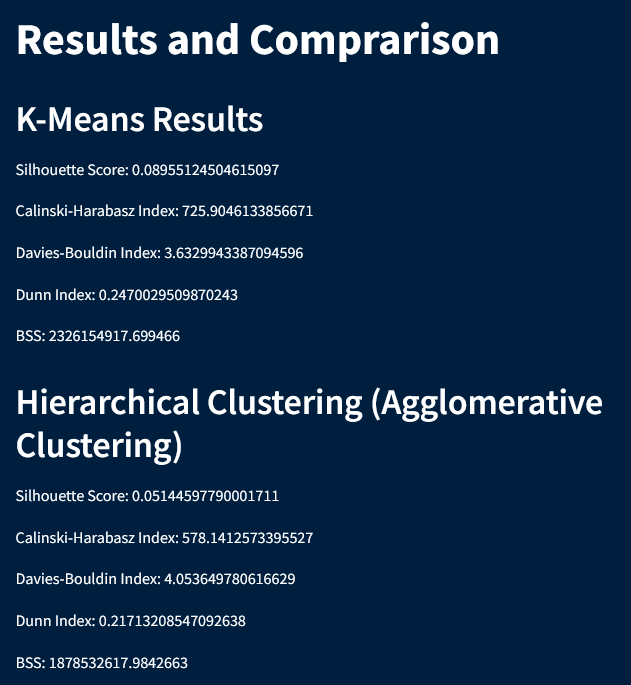
\includegraphics[width=1\linewidth]{clustering-resultsfinal.png}
    \caption{The results from the Clustering Tab}
    \label{fig:clustering-results}
\end{figure}







\end{document}
